\chapter{Topologies}\label{chap:topologies}
The simulations were conducted for six distinct network topologies. Each network has $2^{10}$ (1024) nodes. The behavior of the algorithms in these different topologies is observed, since each topology has different characteristics; different performances exploiting the specials of the topologies are expected. The topologies contain \textit{Complete graph}, \textit{Torus Grid graph}, \textit{Ring graph}, \textit{Star graph}, \textit{Lollipop graph}, and \textit{Ring of Cliques}. In the following, the topologies including these characteristics are presented.

\section{Complete Graph}\label{sec:2completegraph}
The Complete graph $K_N$, as illustrated in \hyperref[fig:completegraphDemo]{figure} \ref{fig:completegraphDemo}, is a graph where each pair of distinct nodes is connected by an edge. The Complete graph, also referred to as a fully connected graph, has $N$ nodes and $\frac{N\times(N-1)}{2}$ edges. The Complete graph is a regular graph, where each node has a degree of $N-1$. As it contains the maximum possible number of edges for a given set of nodes, it is considered a dense graph \cite{GraphTheorySchindelhaauer2021}. The diameter of a Complete graph is 1, as each node is directly connected to every other node. Since each node has the same degree and connectivity, algorithms can treat all nodes uniformly.

The Complete graph is used in financial trading systems and military communications, where high reliability and low latency are critical. The Complete graph ensures optimal routing paths between nodes, due to its low diameter \cite{Banerjee2001}.

\begin{figure}[H]
    \centering
    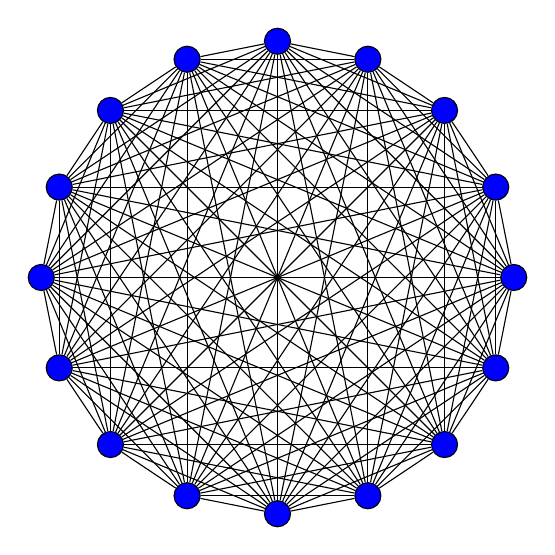
\begin{tikzpicture}
    \foreach \i in {1,...,16} {
      \node[draw, fill=blue, circle, minimum size=4pt] (v\i) at ({360/16 * (\i-1)}:3) {};
    }
    
    \foreach \i in {1,...,16} {
      \foreach \j in {1,...,16} {
        \ifnum\i<\j
          \draw (v\i) -- (v\j);
        \fi
      }
    }
    
  \end{tikzpicture}
    \caption{Complete graph: network size 16}
    \label{fig:completegraphDemo}
\end{figure}
 
\section{Torus Grid Graph}\label{sec:2torusgridgraph}
The two-dimensional Torus Grid graph, also referred to as the $k \times m$-Torus graph or $T_{k,m}$, is a graph that is built like a two-dimensional mesh with wrap-around edges as depicted in \hyperref[fig:torusGraph]{figure} \ref{fig:torusGraph} \cite{Mahlmann2010}. Here, $k$ represents the height, while $m$ denotes the width of the grid. The graph consists of $k \times m$ nodes and $2\times k \times m$ edges (if $k, m$ > 2) and is a regular graph, where each node has a degree of 4. The graph's diameter is given by $\frac{\min(k,m)}{2}$. Tori are scalable, as the number of connections per node is constant, regardless of the graph size. In the previous research \cite{Bayazitoglu}, the simulation results showed to not vary over different network sizes. Torus topology is widely used in supercomputers like IBM Blue Gene and Cray systems for high-performance computing. It is also implemented in Network-on-Chip (NoC) designs for its ability to handle data distribution with low latency and high fault tolerance \cite{Banerjee2001}.

\begin{figure}[H]
    \centering
    \scalebox{1.5}{\tikzset{
    block/.style={draw, fill=blue, circle, minimum size=3pt},
    arrow/.style={->},
    line/.style={-}
}

\begin{tikzpicture}[>=stealth',node distance=0.5cm]
    % Creating rows of blocks
    {[start chain]
        \node[on chain] (s0) {};
        \node[on chain] (s1) {};
        \node[on chain] (s2) {};
        \node[on chain] (s3) {};
        \node[on chain] (s4) {};
    }
    {[start chain]
        \node[block,on chain, below = 0.15 cm of s0] (A0) {};
        \node[block,on chain, join =by {line}] (A1) {};
        \node[block,on chain, join =by {line}] (A2) {};
        \node[block,on chain, join =by {line}] (A3) {};
    }
    {[start chain]
        \node[block,on chain, below = of A0] (B0) {};
        \node[block,on chain, join =by {line}] (B1) {};
        \node[block,on chain, join =by {line}] (B2) {};
        \node[block,on chain, join =by {line}] (B3) {};
    }
    {[start chain]
        \node[block,on chain, below = of B0] (C0) {};
        \node[block,on chain, join =by {line}] (C1) {};
        \node[block,on chain, join =by {line}] (C2) {};
        \node[block,on chain, join =by {line}] (C3) {};
    }
    {[start chain]
        \node[block,on chain, below = of C0] (D0) {};
        \node[block,on chain, join =by {line}] (D1) {};
        \node[block,on chain, join =by {line}] (D2) {};
        \node[block,on chain, join =by {line}] (D3) {};
    }

    % Drawing vertical lines
    \draw (A0) -- (B0) -- (C0) -- (D0); % -- (E0);
    \draw (A1) -- (B1) -- (C1) -- (D1); % -- (E1);
    \draw (A2) -- (B2) -- (C2) -- (D2); % -- (E2);
    \draw (A3) -- (B3) -- (C3) -- (D3); % -- (E3);
    % Drawing loop backs horizontal
    \draw (A0.west) -- ($(A0.west) - (0.15, 0)$);
    \draw ($(A0.west) - (0.15, 0)$) -- ($(A0.west) - (0.15, 0)+(0,0.5)$);
    \draw ($(A0.west) - (0.15, 0)+(0,0.5)$) -- ($(A0.west) +(3.1,0.5)$);
    \draw ($(A0.west) +(3.1,0.5)$) |- (A3.east);
    % \draw (A0.north) |- (s2.north east) -| (A4.north);
    % B row
    \draw (B0.west) -- ($(B0.west) - (0.15, 0)$);
    \draw ($(B0.west) - (0.15, 0)$) -- ($(B0.west) - (0.15, 0)+(0,0.5)$);
    \draw ($(B0.west) - (0.15, 0)+(0,0.5)$) -- ($(B0.west) +(3.1,0.5)$);
    \draw ($(B0.west) +(3.1,0.5)$) |- (B3.east);
    % C row
    \draw (C0.west) -- ($(C0.west) - (0.15, 0)$);
    \draw ($(C0.west) - (0.15, 0)$) -- ($(C0.west) - (0.15, 0)+(0,0.5)$);
    \draw ($(C0.west) - (0.15, 0)+(0,0.5)$) -- ($(C0.west) +(3.1,0.5)$);
    \draw ($(C0.west) +(3.1,0.5)$) |- (C3.east);
    % D row
    \draw (D0.west) -- ($(D0.west) - (0.15, 0)$);
    \draw ($(D0.west) - (0.15, 0)$) -- ($(D0.west) - (0.15, 0)+(0,0.5)$);
    \draw ($(D0.west) - (0.15, 0)+(0,0.5)$) -- ($(D0.west) +(3.1,0.5)$);
    \draw ($(D0.west) +(3.1,0.5)$) |- (D3.east);

    % Vertical Loopbacks

    % 0 column
    \draw (A0.north) -- ($(A0.north) + (0.0, 0.15)$);
    \draw ($(A0.north) + (0, 0.15)$) -- ($(A0.north) + (0, 0.15)+(-0.5,0)$);
    \draw ($(A0.north) + (0, 0.15)+(-0.5,0)$) -- ($(D0.north) +(-0.5,-0.65)$);
    \draw ($(D0.north) +(-0.5,-0.65)$) -| (D0.south);
    % 1 column
    \draw (A1.north) -- ($(A1.north) + (0.0, 0.15)$);
    \draw ($(A1.north) + (0, 0.15)$) -- ($(A1.north) + (0, 0.15)+(-0.5,0)$);
    \draw ($(A1.north) + (0, 0.15)+(-0.5,0)$) -- ($(D1.north) +(-0.5,-0.65)$);
    \draw ($(D1.north) +(-0.5,-0.65)$) -| (D1.south);
    % 2 column
    \draw (A2.north) -- ($(A2.north) + (0.0, 0.15)$);
    \draw ($(A2.north) + (0, 0.15)$) -- ($(A2.north) + (0, 0.15)+(-0.5,0)$);
    \draw ($(A2.north) + (0, 0.15)+(-0.5,0)$) -- ($(D2.north) +(-0.5,-0.65)$);
    \draw ($(D2.north) +(-0.5,-0.65)$) -| (D2.south);

    % 3 column
    \draw (A3.north) -- ($(A3.north) + (0.0, 0.15)$);
    \draw ($(A3.north) + (0, 0.15)$) -- ($(A3.north) + (0, 0.15)+(-0.5,0)$);
    \draw ($(A3.north) + (0, 0.15)+(-0.5,0)$) -- ($(D3.north) +(-0.5,-0.65)$);
    \draw ($(D3.north) +(-0.5,-0.65)$) -| (D3.south);
    
    \end{tikzpicture}}
    \caption{Torus Grid graph: network size 16}
    \label{fig:torusGraph}
\end{figure}

\section{Ring Graph}\label{sec:2ringgraph}
The Ring graph $R_N$ is a regular graph, where each node has a degree of two, forming a cycle. The Ring graph can be constructed by building a Path graph, where the first and the last nodes are connected by an edge as depicted in figure \ref{fig:ring}. The graph consists of $N$ nodes and $N$ edges. The diameter of a ring is given by $\lfloor{\frac{N}{2}}\rfloor$. The regularity ensures that no single node has an advantage, making algorithm design and guaranteeing fairness in load balancing easier. Most of the Ring structures use a token-based communication model. The node that holds the token may transmit data. Most of the current high-speed LANs have a Ring topology \cite{Vidomenko1997}. The advantage of a Ring structure is that it is easy to troubleshoot when faults occur, as the node that is faulty hinders the whole traffic. However, a significant drawback is that a single outage of a node may disrupt the whole network activity.

\begin{figure}[H]
    \centering
    \scalebox{0.8}{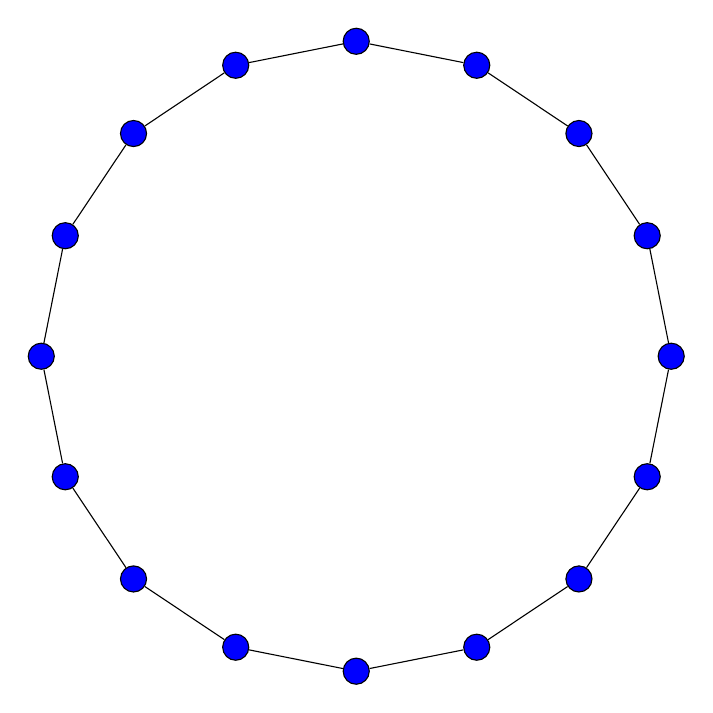
\begin{tikzpicture}
  \def\nodes{16}
  \def\radius{4}
  \foreach \i in {1,...,\nodes} {
      \node[draw, fill=blue, circle, minimum size=6pt] (v\i) 
      at ({\i*360/\nodes}: \radius) {};
  }

  \foreach \i in {1,...,\nodes} {
      \pgfmathtruncatemacro{\j}{mod(\i, \nodes) + 1}
      \draw (v\i) -- (v\j);
  }
\end{tikzpicture}}
    \caption{Ring graph: network size 16}
    \label{fig:ring}
\end{figure}

\section{Star Graph}\label{sec:2stargraph}
A Star graph $S_N$ as illustrated in \hyperref[fig:stargraphDemo]{figure} \ref{fig:stargraphDemo}, is a bipartite graph \cite{west2001introduction} that is structured like a tree structure with a single central node connected to $N-1$ nodes, or leaves. A Star graph with $N$ nodes has $N-1$ edges. In this structure, every leaf node has a degree of 1, meaning it is connected only to the internal node. The central node has a degree of $N-1$. The diameter of a Star graph is 2, as the path from one leaf node through internal node to another leaf node takes two steps. From a load balancing perspective the internal node acts as a point of redistribution. This topology is particularly suitable for master-slave or client-server models where the central node delegates tasks and collects results. A challenge to face when using the Star topology is that the central node may become overloaded in high-load scenarios, requiring careful design to prevent bottlenecks. A common usage for the Star topology is a LAN (Local Area Network) in home networks, where all devices are connected to a hub or the router \cite{Jayeola2023}. A drawback when dealing with Star graphs is that the failure of the central node (hub or router) shuts down the whole network. The advantage of such a setting is that adding new devices is simple and failures of leaf nodes do not affect the whole network.

\begin{figure}[H]
    \centering
    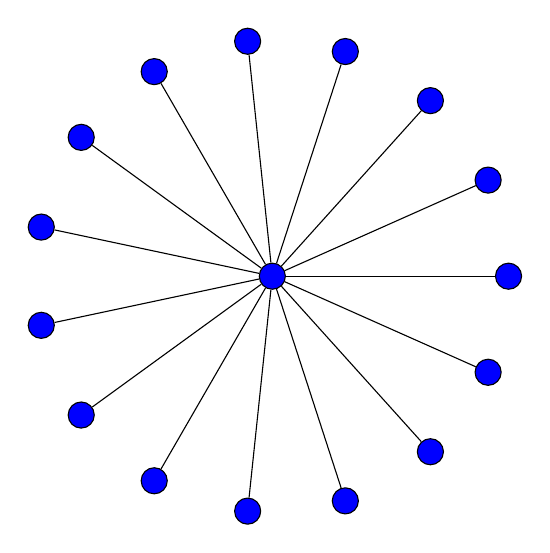
\begin{tikzpicture}
    \node[draw, fill=blue, circle, minimum size=6pt] (center) at (0, 0) {};
    \foreach \i in {1,...,15} {
            \node[draw, fill=blue, circle] (n\i) at ({360/15 * (\i-1)}:3) {};
            \draw (center) -- (n\i);
        }
\end{tikzpicture}
    \caption{Star graph: network size 16}
    \label{fig:stargraphDemo}
\end{figure}


\section{Lollipop Graph}\label{sec:2lollipopgraph}
A $(k, m)$-Lollipop graph $L_{k,m}$ is a graph that consists of a clique and a Path graph as depicted in \hyperref[fig:lollipopgraphDemo]{figure} \ref{fig:lollipopgraphDemo}. The clique and the Path graph are connected by a bridge node, thus a single edge. The $(k, m)$-Lollipop graph consists of a clique with $k$ nodes and a path size of $m$ nodes. A Lollipop graph has $N$ nodes, where $N = k+m$ and $(\frac{k*(k-1)}{2})+m$ edges \cite{JonassonLollipopGraphs2000}.

\begin{figure}[H]
    \centering
    \scalebox{1}{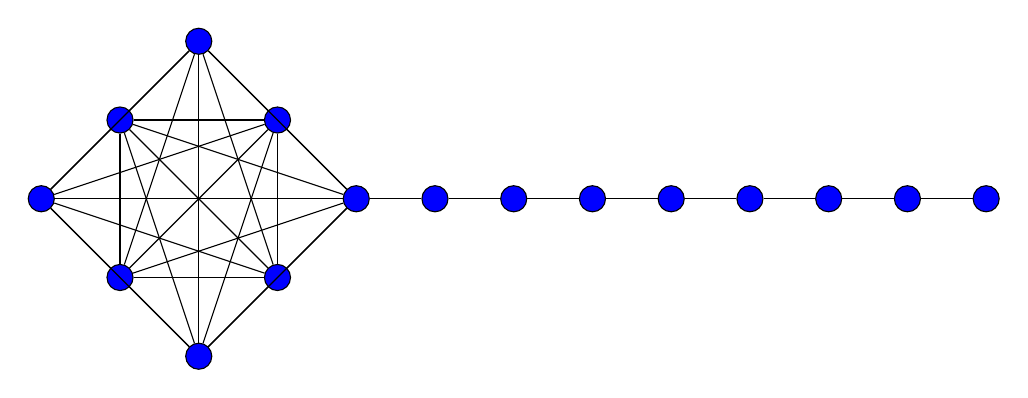
\begin{tikzpicture}
    % Define the 8 vertices in a flat line
    \foreach \i in {1,...,9} {
      \node[draw, fill=blue, circle, minimum size=6pt] (v\i) at (\i, 0) {};
    }
    
    % Draw edges to connect each vertex to the next
    \foreach \i in {1,...,8} {
      \pgfmathtruncatemacro{\j}{\i+1}
      \draw (v\i) -- (v\j);
    }

    % Define additional vertices for the complete graph on v1, centered around v1
    \node[draw, fill=blue, circle, minimum size=6pt] (c1) at (0,1) {};
    \node[draw, fill=blue, circle, minimum size=6pt] (c2) at (0,-1) {};
    \node[draw, fill=blue, circle, minimum size=6pt] (c3) at (-1,2) {};
    \node[draw, fill=blue, circle, minimum size=6pt] (c4) at (-1,-2) {};
    \node[draw, fill=blue, circle, minimum size=6pt] (c5) at (-2,-1) {};
    \node[draw, fill=blue, circle, minimum size=6pt] (c6) at (-2,1) {};
    \node[draw, fill=blue, circle, minimum size=6pt] (c7) at (-3, 0) {};
    
    % Connect the complete graph nodes to v1
    \foreach \k in {1,2,3,4,5,6,7} {
      \draw (v1) -- (c\k);
    }

    % Draw edges between the new nodes to form a complete graph
    \foreach \a in {1,2,3,4,5,6,7} {
      \foreach \b in {\a,...,7} {
        \ifnum\a=\b\else
        \draw (c\a) -- (c\b);
        \fi
      }
    }

  \end{tikzpicture}}
    \caption{Lollipop graph: network size 16}
    \label{fig:lollipopgraphDemo}
\end{figure}

\section{Ring of Cliques}\label{sec:2ringofcliquegraph}
The ($k \times m$)-Ring of Cliques $ROC_{k,m}$ consists of $k$ cliques, each containing $m$ nodes. The cliques are connected to form a ring structure. To create the ring, one edge from each clique is removed, and the endpoints of these removed edges are connected to form a regular graph \cite{Mahlmann2010}. A $k \times m$ ring of cliques has $\left( k\times \left(\frac{m\times (m - 1)}{2}-1 \right) \right)+k$ edges. The connectivity of the graph increases with larger clique sizes and decreases with smaller clique sizes.

\begin{figure}[H]
    \centering
    \scalebox{1}{\newcommand\single[2]{
\foreach \x in {1,...,#2}{
\pgfmathsetmacro{\ang}{360/#2}
    \pgfmathparse{(\x-1)*\ang}
    \node[draw, fill=blue, circle, minimum size=6pt] (#1-\x) at (\pgfmathresult:10cm) {};
  }
  \foreach \x [count=\xi from 1] in {2,4}{
            \foreach \y in {2,4}{
                    \path (#1-\xi) edge[-] (#1-\y);
                    \path (#1-3) edge[-] (#1-\y);
                }
        }
}

\begin{tikzpicture}
    \begin{scope}[local bounding box=scope1]
    \end{scope}

    \foreach \s[count=\si from 0] in {0,90,...,360}{
        \begin{scope}[shift={($(scope1) +(\s:2)$)}, scale=0.1, rotate=\s+90]
            \single{\si}{4};
        \end{scope}
    }

    \foreach \i/\j in {1/2, 2/3, 3/4, 4/1}{
        \ifnum\i=1
            \draw[thick] (\i-1) to[out=180, in=90] (\j-3);
        \else\ifnum\i=2
            \draw[thick] (\i-1) to[out=-90, in=180] (\j-3);
        \else\ifnum\i=3
            \draw[thick] (\i-1) to[out=0, in=-90] (\j-3);
        \else
            \draw[thick] (\i-1) to[out=90, in=0] (\j-3);
        \fi\fi\fi
    }
\end{tikzpicture}

}
    \caption{Ring of Cliques: network size 16}
    \label{fig:ringofcliquesDemo}
\end{figure}

\section{Expected Outcome}\label{sec:expectedoutcome}
\begin{itemize}
    \item \textbf{Complete graph}: The high-connectivity of the Complete graph provides a variety of load transfer opportunities for each node, which will benefit randomized algoithms such as the Push-Pull Sum based load balancing algorithms, as they spread the loads uniformly across the entire network. However, the Complete graph creates a bottleneck for the Deal-Agreement-Based algorithm, as all nodes propose to the same subset of neighbors (if there are multiple nodes that hold $L_{min}$). Since only the highest proposal is accepted per node, the number of transfers per round is significantly limited. 
    \item \textbf{Torus Grid graph}: Many load balancing algorithms perform well on 2D Tori due to the focus on local redistribution. The wrap around edges eliminate boundary effects and provide balanced redistribution across the entire grid. Due to its low regular degree the Deal-Agreement-Based algorithm will perform very well, as the nodes distribute load efficiently between each of its four neighbors. The Adaptive Threshold Push-Pull Sum algorithm improves upon the traditional Push-Pull Sum algorithm by selecting a subset of neighboring nodes and restricting load transfers to those with significant impact on the network balance. This approach utilises smaller neighborhoods more effectively than a purely randomized strategy.
    \item  \textbf{Ring graph}: Unlike Complete graphs or Tori, the Ring graph possesses a sequential nature of data transfers, which makes it slower for loads to propagate across the entire ring. The Deal-Agreement-Based algorithm draws an important advantage over the Push-Pull Based algorithms as it chooses the optimal load transfer partner out of its two immediate neighbors. In contrast, the Push-Pull Sum-based algorithms rely on random neighbor selection, which is suboptimal in a ring structure.The Push-Pull Sum algorithm selects one of two nodes randomly, as does the Adaptive Threshold Push-Pull Sum algorithm, because each node chooses a subset of $\log_{2}{(2)}$ and ultimately ends up with one neighbor.
    \item \textbf{Star graph}: In the Star graph the central node acts as a point of redistribution. This benefits the Push-Pull Sum based algorithms, as each node pushes to the central node (for the Adaptive Threshold Push-Pull Sum algorithm, this is only the case if the load discrepancies surpass the threshold). The central node redistributes loads to each leaf. For the Deal-Agreement-Based algorithm the Star graph creates a bottleneck, since each leaf has only one neighbor (the central node), all nodes propose to the same central node. The internal neighbor initiates the load transfer, accepting the maximal proposing load, resulting in exactly one load transfer.
    \item \textbf{Lollipop graph}: The Lollipop graph is particularly interesting since it combines a dense clique structure with a sparse Path graph, which introduces a mixed topology challenge. The node linking the clique and the Path graph often becomes a bottleneck, since it bridges two different connectivity regions. Within the clique, load balancing is highly efficient for Push-Pull Sum based algorithms, while the Deal-Agreement-Based algorithm struggles due to excessive proposals. Load transfers in the Path graph are sequential, where a deterministic approach like the one of the Deal-Agreement-Based algorithm shows to be very effective, while randomized algorithms like the Push-Pull Sum algorithm will show a moderate perforamce. The relative sizes of the clique and path affect algorithm performance, a larger clique benefits Push-Pull Sum-based approaches, while an extended Path favors the Deal-Agreement-Based algorithm.
    \item \textbf{Ring of Cliques}: Within each clique, Push-Pull Sum-based algorithms perform well due to dense intra-clique connectivity. However, inter-clique balancing poses a challenge for the Push-Pull Sum based algorithms. The Deal-Agreement-Based algorithm benefits from its deterministic load distribution, efficiently transferring loads via the bridging nodes to other cliques once internal balancing is achieved. Push-Pull Sum algorithms struggle due to randomized inter-clique communication. The Adaptive Threshold Push-Pull Sum algorithm mitigates this by selecting neighbors based on a threshold, often favoring inter-clique exchanges, once internal balancing is achieved. The Shared nodes between cliques act as bottlenecks, regulating load transfer and potentially becoming overloaded.
\end{itemize}
